\documentclass{beamer}
\usepackage[utf8]{inputenc}
\usepackage{listings}
\usepackage{tikz}
\usetikzlibrary{positioning,shapes,fit,arrows}
\graphicspath{ {./images/} }

\lstset
{
    language=python,
    breaklines=true,
    basicstyle=\tt\scriptsize,
    keywordstyle=\color{blue},
    identifierstyle=\color{magenta},
}

\usetheme{Antibes}

\usecolortheme{beaver}
\usefonttheme[onlymath]{serif}

% \usecolortheme{crane}
\setbeamertemplate{navigation symbols}{}%remove navigation symbols

\title[Radix Sort---Computer Science Club]{\textbf{Radix Sort}}
% \author{Shon Verch}
\institute{Stephen Lewis Secondary School \\[3ex] {\large Computer Science Club}}
\date{October 26, 2018}

\newcommand{\sectionFrame}[3]
{
    \section{#3}
    \begin{frame}
    \begin{block}{}
    \begin{center}
        \Huge{#1}\\[0.5ex]
        \large{#2}
    \end{center}
    \end{block}
    \end{frame}
}

\begin{document}

\begin{frame} 
\titlepage 
\end{frame} 

\section{Introduction}

\begin{frame}{\textit{Recap...}}
\begin{itemize}
    \item \textbf{Bubble Sort:} $\mathcal{O}(n^2)$
    \item \textbf{Insertion Sort:} $\mathcal{O}(n^2)$
    \item \textbf{Merge Sort:} $\mathcal{O}(n \log(n))$
\end{itemize}
\end{frame}

\begin{frame}{Merge Sort Illustration}
    \begin{figure}
        \centering
        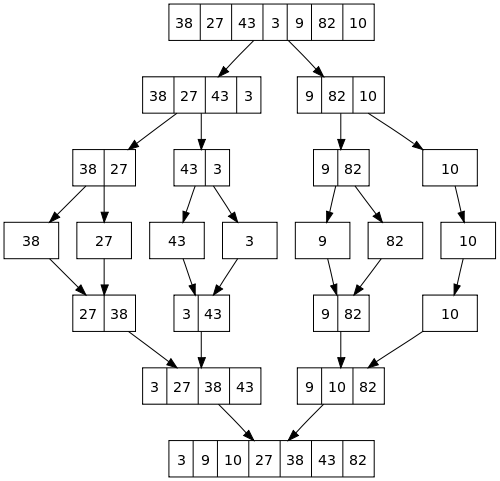
\includegraphics[scale=0.3]{lessons/images/merge_sort.png}
    \end{figure}
\end{frame}

\section{Counting Sort}

\begin{frame}{Brief Explanation of Counting Sort}
Counting sort is an algorithm for sorting a collection of objects according to keys. It works by counting the number of objects that have each distinct key value, and using arithmetic on those counts to determine the positions of each key value in the output sequence.

Counting sort is \textbf{\textit{NOT}} a comparative sorting algorithm; that is, it does not use comparison operations to sort the values.
\end{frame}

\begin{frame}[fragile]{Python Implementation}
\begin{figure}[h]
    \centering
    \begin{lstlisting}
        def sort(values):
            k = len(values)
            count = [0] * k

            for x in values:
                count[x] += 1
            
            total = 0
            for i in range(k):   # i = 0, 1, ... k-1
                old_count = count[i]
                count[i] = total
                total += old_count
            
            output = [0] * k
            for x in values:
                output[count[x)] = x
                count[x] += 1
            
            return output
    \end{lstlisting}
\end{figure}
\end{frame}

\section{Radix Sort}

\begin{frame}{What is it?}
Radix sort is simply an \textit{extension} of counting sort. It works by sorting the digits of the values successively.

\begin{figure}
    \centering
    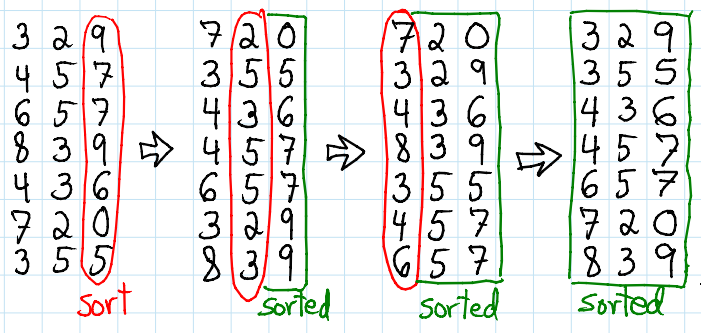
\includegraphics[width=\textwidth]{lessons/images/radix_sort.png}
\end{figure}

\end{frame}

\end{document}

